\documentclass[11pt,letterpaper]{article}
\usepackage[margin=0.9in]{geometry}
\usepackage[T1]{fontenc}
\usepackage[utf8]{inputenc}
\usepackage{newtxtext,newtxmath}
\usepackage{microtype}
\usepackage{amsmath}
\usepackage{graphicx}
\usepackage{booktabs,tabularx,array}
\usepackage{caption}
\usepackage{titlesec}
\usepackage{placeins}
\usepackage[hidelinks]{hyperref}
\captionsetup{font=small,labelfont=bf,labelsep=period,skip=5pt}
\titleformat{\section}{\large\bfseries}{\thesection}{0.7em}{}
\titleformat{\subsection}{\normalsize\bfseries}{}{0pt}{}
\titlespacing*{\section}{0pt}{12pt plus 2pt minus 1pt}{6pt}
\titlespacing*{\subsection}{0pt}{8pt plus 1pt}{4pt}
\setlength{\parindent}{0pt}
\setlength{\parskip}{5pt plus 1pt minus 1pt}
\setlength{\textfloatsep}{11pt plus 2pt minus 2pt}
\setlength{\floatsep}{10pt plus 2pt minus 2pt}
\setlength{\intextsep}{10pt plus 2pt minus 2pt}
\setlength{\abovedisplayskip}{7pt plus 2pt minus 2pt}
\setlength{\belowdisplayskip}{7pt plus 2pt minus 2pt}
\renewcommand{\topfraction}{0.92}
\renewcommand{\bottomfraction}{0.85}
\renewcommand{\textfraction}{0.07}
\renewcommand{\floatpagefraction}{0.8}
\setcounter{topnumber}{3}
\setcounter{bottomnumber}{2}
\setcounter{totalnumber}{4}
\widowpenalty=10000
\clubpenalty=10000
\emergencystretch=1.5em
\newcommand{\sym}[1]{\textsuperscript{#1}}
\newcommand{\vname}[1]{\texttt{#1}}
\hypersetup{pdftitle={Learning from Success and Failure in Formula One},pdfsubject={ISOM 753 Assignment 3},pdfcreator={LaTeX}}

\begin{document}
\begin{center}
{\Large\bfseries Learning from Success and Failure in Formula One}\par
\vspace{4pt}
{\normalsize ISOM 753 Assignment 3}
\end{center}
\vspace{-3pt}

\section{Research Question and Contribution}

How individuals learn from past success and failure matters for understanding performance improvement. The value of experience may depend on whether it comes from one's own outcomes or those of others, and on the setting in which those outcomes occur. Lapr\'{e} and Cravey (2022) study Formula One (F1) racing to ask which experiences help individuals win when success is rare and competitive. Each race has one winner, whose success prevents every other driver from winning. Mechanical problems, accidents and collisions can also force drivers to retire. Drivers must make use of limited winning experience and assess what they can learn from different kinds of failure.

The original study uses 21,487 driver--race observations from 1950--2017. It relates the experience accumulated by a driver and through teammates before a race to the driver's chance of winning that race. The authors find an inverted-U relationship between total racing experience and winning, so the benefits of experience do not increase indefinitely with starts. When experience is separated by source, own wins, teammate wins and own car failures are positively associated with later wins. Own driver failures do not show the same positive relationship. The number of races entered therefore gives an incomplete account of individual learning. What happened in those races, and whether the driver experienced it personally or through a teammate, also matters.

The authors explain these findings through learning opportunities and the way failures are analyzed. Own wins are scarce, so teammates' successes provide additional opportunities to learn about effective car setups and race strategies. Engine, gearbox and suspension failures can often be traced through technical inspections and post-race analysis. Drivers may learn to recognize abnormal car behavior, adjust their driving and protect the car. Driver failures more readily raise questions of blame. Drivers may attribute an accident to another competitor or external conditions and spend less effort examining their own behavior. Different types of failure may therefore produce different learning outcomes.

The frequency of car failures is an important condition in this argument. Repeated failures give drivers opportunities to encounter problems, investigate causes and adjust their behavior. Finishing is also a prerequisite for winning. This environment has changed in more recent F1 seasons. Under this study's classification, car failures account for about 37.8\% of starts in 1970--1989, compared with about 7.1\% in 2018--2025. Winning remains scarce and competitive, but drivers now have far fewer opportunities to experience car failures. The extension asks whether learning from own car failures weakens when those failures become less common.

The analysis first reconstructs cumulative experience from the race-level records in the authors' Excel workbook, checks the results against their Stata data and replicates Table 1 and models (1), (2) and (4) of Table 2. It then adds the 2018--2025 seasons and estimates model (4) on the full 1950--2025 sample and on 2018--2025 alone. Drivers who raced before 2018 carry their accumulated success and failure experience into the extension. Their histories do not restart at zero.

This extension examines the authors' explanation about failure frequency across periods within the same sport. F1 still has only one race winner, but car failures are much less common. The comparison asks whether the experience relationships in the original study hold under that change in conditions.

\section{Empirical Setting and Data}

The analysis uses race-level F1 data to study the relationship between prior success and failure experience and subsequent wins. The historical data come from the authors' Excel workbook and cover 1950--2017. Applying the original sample rules leaves 21,487 driver--race observations across 965 races. The extension uses the Jolpica API and covers 173 Grands Prix from 2018--2025, adding 3,440 actual starts. The combined estimation panel contains 24,927 observations.

The original study defines experience as the relevant events accumulated before the current race begins. This replication follows that definition and reconstructs cumulative variables from participation, win and retirement flags. Each race first contributes an event count to the driver's history. Those counts are then summed over all earlier races. For driver $i$ before race $r$, cumulative experience of a given type is
\[
C_{ir}=\sum_{s<r}e_{is},
\]
where $e_{is}$ is the experience increment from an earlier race $s$. For an ordinary record with one driver and one car, the counting rules are given below.

\begin{center}
\small
\renewcommand{\arraystretch}{1.08}
\begin{tabularx}{\linewidth}{@{}l>{\raggedright\arraybackslash}X>{\raggedright\arraybackslash}p{0.33\linewidth}@{}}
\toprule
Variable & Increment from the current race & Cumulative value before the race \\
\midrule
\vname{crace} & One for an actual start. Nonstarts do not count. & Number of prior starts. \\
\vname{cw} & One for an own win, zero otherwise. & Number of prior own wins. \\
\vname{ctw} & Winning shares of other drivers on the same team in the same race. The focal driver's win is excluded. & Sum of teammate winning shares from earlier races entered together. \\
\vname{cfc} & One for an own car-failure event, including a technical disqualification. & Number of prior own car failures. \\
\vname{cfd} & One for an own driver-failure event, including a sporting disqualification. & Number of prior own driver failures. \\
\vname{ctfc} & Car-failure events of other drivers on the same team in the same race. & Sum of teammate car failures from earlier races entered together. \\
\vname{ctfd} & Driver-failure events of other drivers on the same team in the same race. & Sum of teammate driver failures from earlier races entered together. \\
\bottomrule
\end{tabularx}
\end{center}


A race outcome changes the experience variables used in later races. It does not enter that race's own explanatory variables. Failing to win is not automatically a failure. A driver who finishes without winning gains racing experience but no car- or driver-failure increment. Teammate car and driver failures use the same event-counting and prior-accumulation method.

Early shared drives require further adjustments because the workbook records driver--car--race observations. A driver can have several rows in one race. Following the authors, each row contributes $1/\vname{ncs}$ starts, where \vname{ncs} is the number of cars driven by that driver in that race. Summing these shares within a driver--race still gives one start. Winning experience is calculated as $\vname{win}/\vname{nds}$, where \vname{nds} is the number of drivers sharing the car. This allocates a shared win across its drivers. Teammate wins are calculated by summing winning shares within the team and race, adjusting for multiple-car drives and subtracting the focal driver's share. Experience is constructed using all original rows before observations with $\vname{ncs}>1$ are excluded from estimation. Their contribution to later histories is therefore retained. The reconstructed cumulative variables match the authors' Stata data row by row.

Teammate experience also follows the original definition. A teammate's outcome counts only when the focal driver participates in the same race for the same team. Drivers retain experience after changing teams. A new teammate's achievements before they raced together are not added retrospectively. The measure captures teammate experience encountered while racing together, rather than the current teammate's entire career record.

The extension uses the same calculation and appends races after 2017 to the historical records. Returning drivers begin with their closing experience balances through 2017. First-time drivers begin at zero. Entries recorded as pre-race withdrawals with zero completed laps are excluded from starts and experience histories. Retirement flags are initially based on the API's \vname{status} field. Explicit mechanical and component problems are classified as car failures. Accidents, collisions and driving-related causes are classified as driver failures. Disqualifications are classified by cause, with technical violations coded as car failures and sporting violations as driver failures. Race reports are checked when a status such as \vname{Retired} does not identify the cause. Applying the status rule to historical data gives 93.63\% agreement among linked observations that the authors coded as retirements, counting unclassified outcomes as disagreements. Wet weather and track type in the new seasons are coded manually from Wikipedia race reports, following the original approach.

\section{Research Design and Identification}

The dependent variable indicates whether a driver wins the current race. Binary logit models replicate models (1), (2) and (4) in the original Table 2. The specifications use the same outcome and controls but represent experience differently and differ in whether team indicators are included. Model (1) includes cumulative starts and their square. Model (2) replaces the linear starts term with own wins, teammate wins, own car failures, own driver failures and the two types of teammate failure. Squared starts remain in the model. Model (4) adds the authors' 20 team indicators.

For model (4), let $p_{ir}$ denote the probability that driver $i$ wins race $r$. The original specification is
\[
\log\left(\frac{p_{ir}}{1-p_{ir}}\right)
=\alpha+\boldsymbol{\beta}'\mathbf{E}_{ir}
+\delta\,\mathrm{crace}_{ir}^{2}
+\boldsymbol{\gamma}'\mathbf{X}_{ir}
+\boldsymbol{\theta}'\mathbf{D}_{ir}+u_r.
\]
The vector $\mathbf{E}_{ir}$ contains the six pre-race cumulative experience measures \vname{cw}, \vname{ctw}, \vname{cfc}, \vname{cfd}, \vname{ctfc} and \vname{ctfd}. Controls in $\mathbf{X}_{ir}$ include grid position, age, home race, wet weather, track type and the number of actual starters. The vector $\mathbf{D}_{ir}$ contains the team indicators. Teams not covered by these indicators form the reference group.

These controls distinguish experience from other competitive conditions. Grid position reflects qualifying performance before the current race. Age accounts for differences associated with career stage. Weather, track type and field size describe the race environment. Team indicators account for average differences between the teams identified in the original study. The experience coefficients thus measure the relationship between past experience and winning conditional on these variables. They are in log-odds units and do not directly measure percentage-point changes in winning probability.

Following the original method, the models first include a race random intercept $u_r$ and are estimated with \vname{lme4::glmer}. The estimated race-intercept variance is close to zero in the historical and extension models. The maximum difference between the fixed coefficients and ordinary logit is below $2\times10^{-6}$. The reported results therefore use ordinary logit with standard errors clustered by race, allowing observations from the same race to be correlated.

The extension applies model (4) to 1950--2025 and to 2018--2025 separately, retaining the variable definitions and model structure. All experience coefficients are reported in the findings. Williams has no wins in the modern sample, so its indicator perfectly predicts non-winning. Its 343 observations are excluded only from the modern regression, and indicators that are constant within that subsample are removed. This leaves 3,097 estimation observations. The excluded records remain in the experience histories, preserving their contribution to later races and to teammate experience.

Car failures are much less common in 2018--2025. To test whether prior car-failure experience has a weaker relationship with later winning in this setting, the analysis compares the \vname{cfc} coefficients from the historical and modern samples. Every parameter in model (4) is estimated separately in each period. The difference is
\[
\Delta=\widehat{\beta}_{cfc,\,2018\text{--}2025}
-\widehat{\beta}_{cfc,\,1950\text{--}2017}.
\]
The periods share no race clusters. Under race-clustered inference, the standard error of the difference is
\[
SE(\Delta)=\sqrt{
SE\!\left(\widehat{\beta}_{cfc,\,2018\text{--}2025}\right)^2
+SE\!\left(\widehat{\beta}_{cfc,\,1950\text{--}2017}\right)^2}.
\]
A weaker relationship corresponds to $\Delta<0$. The analysis reports a one-sided test in that direction, a two-sided difference test and a 95\% confidence interval. The 1950--2025 estimate describes the overall relationship after the new seasons are added. The period comparison uses the non-overlapping historical and modern samples.

Experience coefficients use differences across drivers and changes within a driver's career. Experience is not randomly assigned. Ability, access to competitive cars and career selection may remain correlated with cumulative experience, so the estimates are interpreted as conditional associations. The historical and modern periods also differ in technology and rules. Comparing periods can test whether the modern relationship is weaker, but it cannot attribute any difference solely to the decline in car-failure frequency.

\section{Findings and Mechanism}

Table~\ref{tab:descriptive} compares the published descriptive statistics with the independently reconstructed results. Every statistic matches at the precision reported in the paper, and the cumulative variables match the authors' Stata data row by row. The historical win rate is 4.48\%, so winning is rare. Drivers enter a race with an average of 3.81 own wins and 16.69 own car failures. Car failures thus provide far more experience than own wins in the original setting.

\begin{table}[!htbp]
\centering
\caption{Published and replicated descriptive statistics}
\label{tab:descriptive}
\fontsize{8.5}{10}\selectfont
\setlength{\tabcolsep}{2pt}
\renewcommand{\arraystretch}{1.08}
\begin{tabular*}{\linewidth}{@{\extracolsep{\fill}}lrrrrrrrr@{}}
\toprule
 & \multicolumn{4}{c}{Published} & \multicolumn{4}{c}{R replication} \\
\cmidrule(lr){2-5}\cmidrule(l){6-9}
Variable & Mean & SD & Min & Max & Mean & SD & Min & Max \\
\midrule
Win & 0.0448 & 0.2069 & 0 & 1 & 0.0448 & 0.2069 & 0 & 1 \\
Podium & 0.1342 & 0.3406 & 0 & 1 & 0.1342 & 0.3406 & 0 & 1 \\
Prior starts & 59.85 & 59.86 & 0 & 321 & 59.85 & 59.86 & 0 & 321 \\
Own wins & 3.81 & 9.72 & 0 & 91 & 3.81 & 9.72 & 0 & 91 \\
Teammate wins & 3.27 & 6.73 & 0 & 55 & 3.27 & 6.73 & 0 & 55 \\
Own car failures & 16.69 & 17.03 & 0 & 113 & 16.69 & 17.03 & 0 & 113 \\
Own driver failures & 7.26 & 7.52 & 0 & 39 & 7.26 & 7.52 & 0 & 39 \\
Teammate car failures & 15.69 & 16.29 & 0 & 92 & 15.69 & 16.29 & 0 & 92 \\
Teammate driver failures & 7.30 & 8.27 & 0 & 45 & 7.30 & 8.27 & 0 & 45 \\
Grid position & 11.96 & 6.84 & 1 & 34 & 11.96 & 6.84 & 1 & 34 \\
Age & 30.13 & 5.14 & 17.46 & 55.80 & 30.13 & 5.14 & 17.46 & 55.80 \\
Home race & 0.0828 & 0.2756 & 0 & 1 & 0.0828 & 0.2756 & 0 & 1 \\
Wet weather & 0.1575 & 0.3643 & 0 & 1 & 0.1575 & 0.3643 & 0 & 1 \\
Permanent track & 0.7301 & 0.4439 & 0 & 1 & 0.7301 & 0.4439 & 0 & 1 \\
Occasional track & 0.1534 & 0.3604 & 0 & 1 & 0.1534 & 0.3604 & 0 & 1 \\
Number of starters & 22.83 & 3.03 & 6 & 34 & 22.83 & 3.03 & 6 & 34 \\
\bottomrule
\end{tabular*}
\par\vspace{4pt}\begin{minipage}{\linewidth}\footnotesize
Both versions use 21,487 observations. Values are displayed at the original paper's precision. All reported statistics match.
\end{minipage}
\end{table}


Table~\ref{tab:replication} compares the published estimates with the re-estimated models (1), (2) and (4). Coefficients, standard errors and significance agree at the published precision. Model (1) has a positive coefficient on cumulative starts and a negative coefficient on squared starts, indicating a relationship that first rises and then falls. After model (2) separates success and failure experience, own wins, teammate wins and own car failures are all positive and significant.

With team indicators included in model (4), the coefficients on own wins, teammate wins, own car failures and teammate driver failures are 0.0426, 0.0175, 0.0189 and 0.0269. All are positive and significant at 5\%. Conditional on the other variables, drivers with more of these four types of experience have higher odds of winning later races. The teammate-win coefficient falls from 0.0280 in model (2) to 0.0175 but remains positive and significant.

The other two experience measures are not significant. Own driver failures and teammate car failures have coefficients of $-0.0135$ and $-0.0066$. The model does not detect a significant association between either measure and subsequent wins.

\begin{table}[!htbp]
\centering
\caption{Replication of the original Table 2}
\label{tab:replication}
\fontsize{8.5}{10}\selectfont
\setlength{\tabcolsep}{3pt}
\renewcommand{\arraystretch}{1.10}
\begin{tabular*}{\linewidth}{@{\extracolsep{\fill}}lrrrrrr@{}}
\toprule
 & \multicolumn{2}{c}{Model (1)} & \multicolumn{2}{c}{Model (2)} & \multicolumn{2}{c}{Model (4)} \\
\cmidrule(lr){2-3}\cmidrule(lr){4-5}\cmidrule(l){6-7}
Variable & Published & R & Published & R & Published & R \\
\midrule
Prior starts & \shortstack[r]{$0.0118^{***}$\\{\scriptsize (0.0018)}} & \shortstack[r]{$0.0118^{***}$\\{\scriptsize (0.0018)}} & {--} & {--} & {--} & {--} \\
Own wins & {--} & {--} & \shortstack[r]{$0.0416^{***}$\\{\scriptsize (0.0040)}} & \shortstack[r]{$0.0416^{***}$\\{\scriptsize (0.0040)}} & \shortstack[r]{$0.0426^{***}$\\{\scriptsize (0.0043)}} & \shortstack[r]{$0.0426^{***}$\\{\scriptsize (0.0043)}} \\
Teammate wins & {--} & {--} & \shortstack[r]{$0.0280^{***}$\\{\scriptsize (0.0073)}} & \shortstack[r]{$0.0280^{***}$\\{\scriptsize (0.0073)}} & \shortstack[r]{$0.0175^{*}$\\{\scriptsize (0.0078)}} & \shortstack[r]{$0.0175^{*}$\\{\scriptsize (0.0078)}} \\
Own car failures & {--} & {--} & \shortstack[r]{$0.0162^{**}$\\{\scriptsize (0.0054)}} & \shortstack[r]{$0.0162^{**}$\\{\scriptsize (0.0054)}} & \shortstack[r]{$0.0189^{**}$\\{\scriptsize (0.0062)}} & \shortstack[r]{$0.0189^{**}$\\{\scriptsize (0.0062)}} \\
Own driver failures & {--} & {--} & \shortstack[r]{$-0.0223$\\{\scriptsize (0.0116)}} & \shortstack[r]{$-0.0223$\\{\scriptsize (0.0116)}} & \shortstack[r]{$-0.0135$\\{\scriptsize (0.0125)}} & \shortstack[r]{$-0.0135$\\{\scriptsize (0.0125)}} \\
Teammate car failures & {--} & {--} & \shortstack[r]{$-0.0059$\\{\scriptsize (0.0049)}} & \shortstack[r]{$-0.0059$\\{\scriptsize (0.0049)}} & \shortstack[r]{$-0.0066$\\{\scriptsize (0.0052)}} & \shortstack[r]{$-0.0066$\\{\scriptsize (0.0052)}} \\
Teammate driver failures & {--} & {--} & \shortstack[r]{$0.0219^{*}$\\{\scriptsize (0.0089)}} & \shortstack[r]{$0.0219^{*}$\\{\scriptsize (0.0089)}} & \shortstack[r]{$0.0269^{**}$\\{\scriptsize (0.0095)}} & \shortstack[r]{$0.0269^{**}$\\{\scriptsize (0.0095)}} \\
Prior starts squared & \shortstack[r]{$-0.00004^{***}$\\{\scriptsize (0.00001)}} & \shortstack[r]{$-0.00004^{***}$\\{\scriptsize (0.00001)}} & \shortstack[r]{$-0.00004^{***}$\\{\scriptsize (0.00001)}} & \shortstack[r]{$-0.00004^{***}$\\{\scriptsize (0.00001)}} & \shortstack[r]{$-0.00006^{***}$\\{\scriptsize (0.00001)}} & \shortstack[r]{$-0.00006^{***}$\\{\scriptsize (0.00001)}} \\
Team indicators & No & No & No & No & Yes & Yes \\
Grid position & \shortstack[r]{$-0.5209^{***}$\\{\scriptsize (0.0243)}} & \shortstack[r]{$-0.5209^{***}$\\{\scriptsize (0.0243)}} & \shortstack[r]{$-0.4798^{***}$\\{\scriptsize (0.0236)}} & \shortstack[r]{$-0.4798^{***}$\\{\scriptsize (0.0236)}} & \shortstack[r]{$-0.4388^{***}$\\{\scriptsize (0.0242)}} & \shortstack[r]{$-0.4388^{***}$\\{\scriptsize (0.0242)}} \\
Age & Yes & Yes & Yes & Yes & Yes & Yes \\
Home race & Yes & Yes & Yes & Yes & Yes & Yes \\
Wet weather & Yes & Yes & Yes & Yes & Yes & Yes \\
Permanent track & Yes & Yes & Yes & Yes & Yes & Yes \\
Occasional track & Yes & Yes & Yes & Yes & Yes & Yes \\
Number of starters & Yes & Yes & Yes & Yes & Yes & Yes \\
Constant & Yes & Yes & Yes & Yes & Yes & Yes \\
Wald $\chi^2$ & $642.30^{***}$ & $642.30^{***}$ & $863.91^{***}$ & $863.91^{***}$ & $915.82^{***}$ & $915.82^{***}$ \\
Observations & 21,487 & 21,487 & 21,487 & 21,487 & 21,487 & 21,487 \\
\bottomrule
\end{tabular*}
\par\vspace{4pt}\begin{minipage}{\linewidth}\footnotesize
Coefficients are in log-odds units. Standard errors clustered by race are in parentheses.
$^{*}p<0.05$, $^{**}p<0.01$, $^{***}p<0.001$. A dash indicates a variable omitted from the specification.
\end{minipage}
\end{table}


Figure~\ref{fig:failure-rates} shows annual failure rates from 1950--2025. Car failures were common in earlier races and became less frequent over time. Their rate falls from 37.79\% in 1970--1989 to 7.12\% in 2018--2025. Each rate is the number of failures divided by actual starts. Modern racing therefore provides a setting with fewer car failures in which to examine the original argument about frequent failure and learning opportunities.

\begin{figure}[!htbp]
\centering
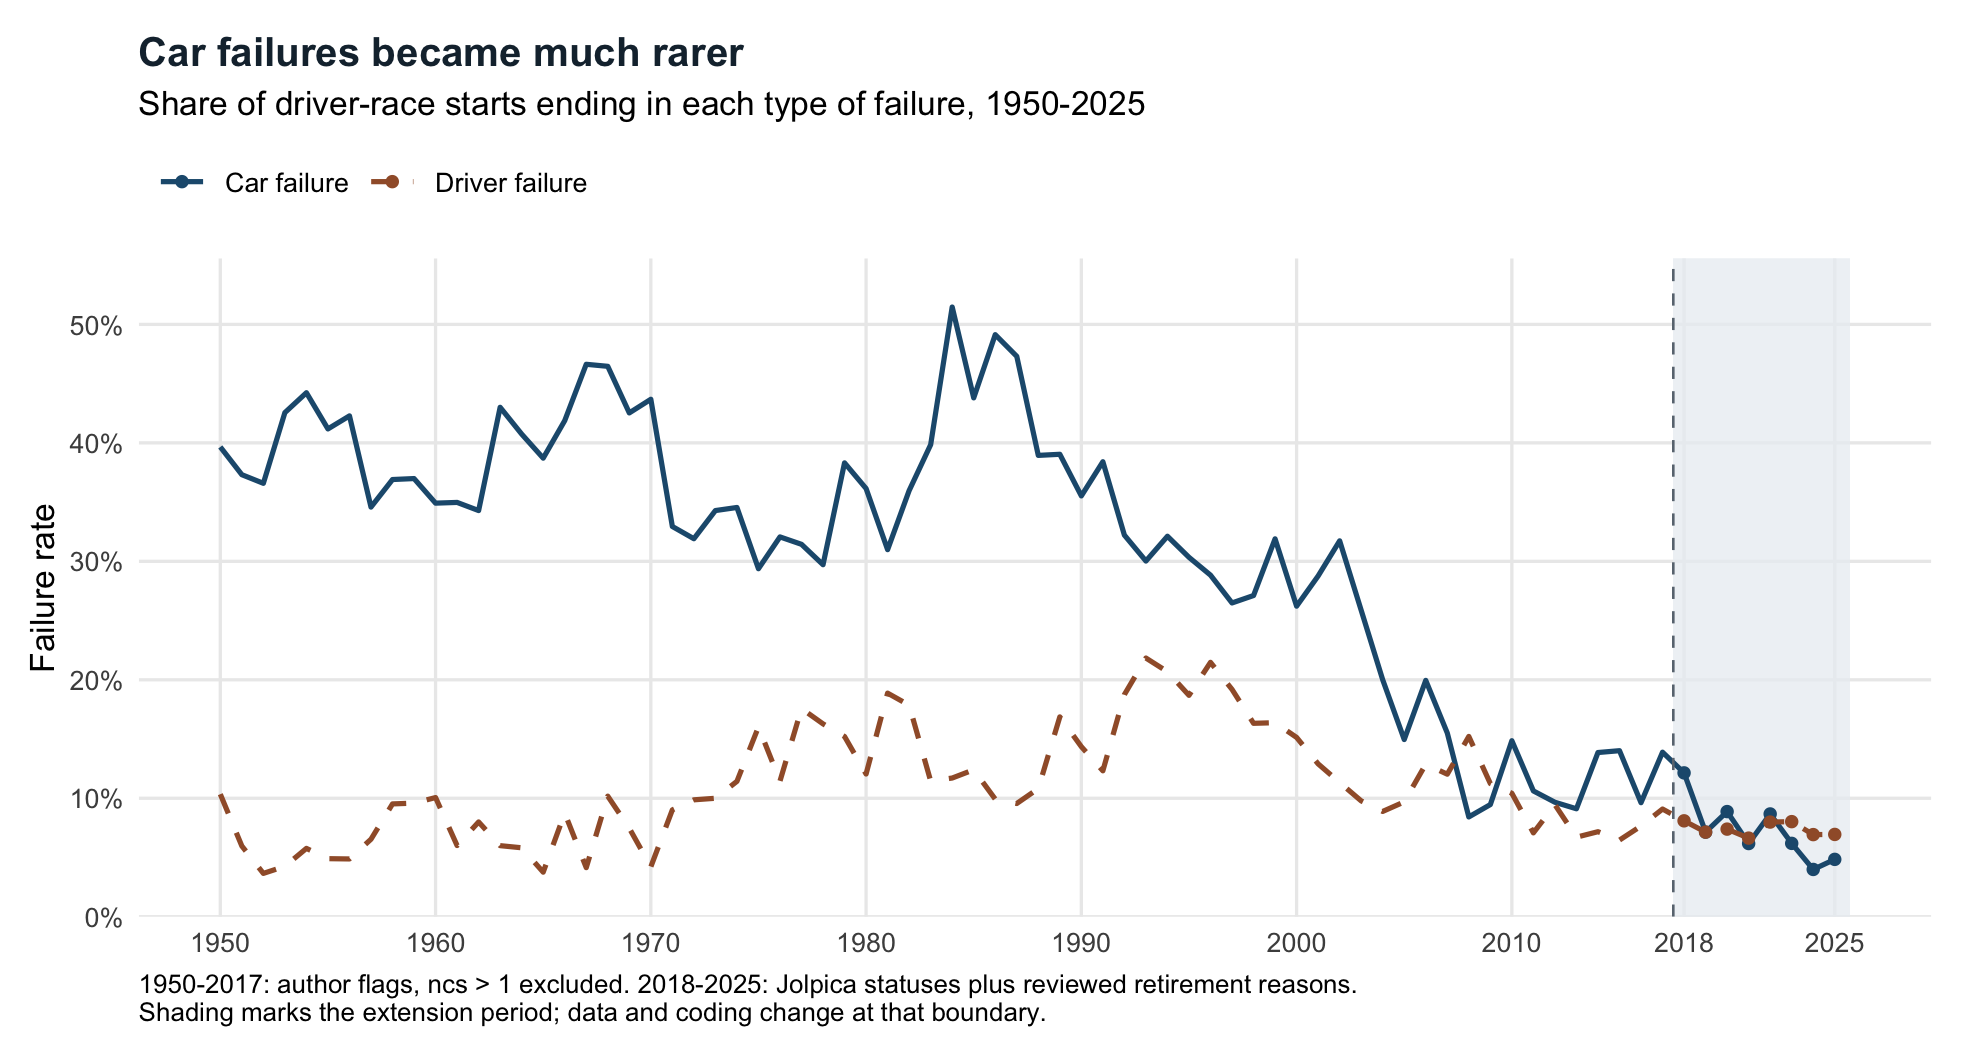
\includegraphics[width=\linewidth]{figures/figure1_failure_rates.png}
\caption{Annual car- and driver-failure rates, 1950--2025}
\label{fig:failure-rates}
\vspace{-2pt}
\begin{minipage}{\linewidth}\footnotesize
Rates are calculated from actual-start records. The figure uses the authors' historical event flags and the reviewed extension classifications. Records excluded only from the modern regression remain in the rate calculations.
\end{minipage}
\end{figure}

Table~\ref{tab:extension} compares the 1950--2025 and 2018--2025 estimates with model (4) for the original 1950--2017 period. The positive association between own winning experience and later wins remains, but failure and teammate experience show different patterns.

\subsection*{Own wins remain significant and teammate car failures remain insignificant}

Own winning experience is positive and significant in all three samples. The full-sample coefficient is close to the original 1950--2017 estimate. The modern estimate is smaller but remains positive and significant. The original study argues that wins help drivers develop race tactics, manage pace while leading and look after the car. These skills concern how to complete a winning race as well as how to avoid mechanical trouble. Even with improved reliability, the judgment and execution learned from success may remain valuable. The extension is consistent with this explanation.

Teammate car failures do not reach 5\% significance in any of the three samples. There are two possible explanations. Recognizing unusual sounds and sensing the car's condition involve tacit knowledge that may be difficult to convey to a teammate. Drivers may also have enough own car-failure experience to have little need to learn from a teammate's failures. With fewer car failures in 2018--2025, the second explanation is less persuasive than in the original setting, although the difficulty of transferring that knowledge may remain.

\subsection*{Driver failures become significant in the modern sample}

The clearest change concerns own driver failures. In the original 1950--2017 model (4), the coefficient is $-0.0135$ and insignificant. It is also insignificant in the full 1950--2025 sample. In 2018--2025, however, the coefficient is 0.1594 and positive and significant.

The original theory predicts less learning from driver failures than from car failures. Accidents and collisions raise questions of responsibility. Drivers may blame opponents, luck or other external factors and have less incentive to reflect or change their behavior. Car failures have a range of technical causes that more readily support root-cause analysis.

In the modern sample, own driver-failure experience is positively associated with later winning. One possible explanation is that, as mechanical failures decline, judging overtaking opportunities, avoiding collisions and controlling race risk become more important. Experience gained from past driver failures may then be more valuable. Another explanation concerns who remains in the sample. Drivers with longer careers have more opportunities to accumulate accidents. Those who stay in F1 may also be more competitive. The modern association may therefore reflect both learning after accidents and the ability of drivers who continue racing for longer.

Own car failures are positive and significant in the original 1950--2017 model (4), with a coefficient of 0.0189. The full-sample coefficient falls to 0.0113, with $p=0.0516$, just above the 5\% threshold. The modern coefficient is 0.0127, with $p=0.8156$, and is also insignificant. Its point estimate is below the original estimate but is imprecise. The estimated change is $-0.0062$, with a 95\% confidence interval of $[-0.1137,\,0.1013]$. The two-sided difference test gives $p=0.9100$, and the one-sided test for weakening gives $p=0.4550$. There is therefore insufficient evidence that learning from own car failures has weakened.

Teammate wins and teammate driver failures are positive and significant in the original model (4) but do not reach 5\% significance in either extension sample. The authors explain the value of teammate success through the extra winning experience it supplies and the similar technical conditions within a team, which help drivers understand and adopt successful setups. The extension does not provide the same support. The modern period contains fewer races, and teammate-experience estimates are less precise. Teammate wins also vary with team competitiveness, making their independent relationships harder to distinguish. Teammate driver failures already become insignificant when the original paper adds champion-driver controls in its Table 3, so this result is sensitive to the specification.

\begin{table}[!htbp]
\centering
\caption{Model (4) in the original and extension samples}
\label{tab:extension}
\small
\setlength{\tabcolsep}{5pt}
\renewcommand{\arraystretch}{1.10}
\begin{tabular*}{\linewidth}{@{\extracolsep{\fill}}lrrr@{}}
\toprule
Variable & 1950--2017 & 1950--2025 & 2018--2025 \\
\midrule
Own wins & \shortstack[r]{$0.0426^{***}$\\{\scriptsize (0.0043)}} & \shortstack[r]{$0.0409^{***}$\\{\scriptsize (0.0037)}} & \shortstack[r]{$0.0290^{***}$\\{\scriptsize (0.0083)}} \\
Teammate wins & \shortstack[r]{$0.0175^{*}$\\{\scriptsize (0.0078)}} & \shortstack[r]{$0.0073$\\{\scriptsize (0.0058)}} & \shortstack[r]{$0.0093$\\{\scriptsize (0.0176)}} \\
Own car failures & \shortstack[r]{$0.0189^{**}$\\{\scriptsize (0.0062)}} & \shortstack[r]{$0.0113$\\{\scriptsize (0.0058)}} & \shortstack[r]{$0.0127$\\{\scriptsize (0.0545)}} \\
Own driver failures & \shortstack[r]{$-0.0135$\\{\scriptsize (0.0125)}} & \shortstack[r]{$0.0047$\\{\scriptsize (0.0113)}} & \shortstack[r]{$0.1594^{**}$\\{\scriptsize (0.0516)}} \\
Teammate car failures & \shortstack[r]{$-0.0066$\\{\scriptsize (0.0052)}} & \shortstack[r]{$-0.0020$\\{\scriptsize (0.0050)}} & \shortstack[r]{$0.0218$\\{\scriptsize (0.0474)}} \\
Teammate driver failures & \shortstack[r]{$0.0269^{**}$\\{\scriptsize (0.0095)}} & \shortstack[r]{$0.0088$\\{\scriptsize (0.0075)}} & \shortstack[r]{$-0.0898$\\{\scriptsize (0.0554)}} \\
Prior starts squared & \shortstack[r]{$-0.00006^{***}$\\{\scriptsize (0.00001)}} & \shortstack[r]{$-0.00004^{***}$\\{\scriptsize (0.00001)}} & \shortstack[r]{$-0.00007^{***}$\\{\scriptsize (0.00002)}} \\
Team indicators & Yes & Yes & Yes \\
Grid position & \shortstack[r]{$-0.4388^{***}$\\{\scriptsize (0.0242)}} & \shortstack[r]{$-0.4514^{***}$\\{\scriptsize (0.0238)}} & \shortstack[r]{$-0.4877^{***}$\\{\scriptsize (0.0998)}} \\
Age & Yes & Yes & Yes \\
Home race & Yes & Yes & Yes \\
Wet weather & Yes & Yes & Yes \\
Permanent track & Yes & Yes & Yes \\
Occasional track & Yes & Yes & Yes \\
Number of starters & Yes & Yes & Yes \\
Constant & Yes & Yes & Yes \\
Observations & $21,487$ & $24,927$ & $3,097$ \\
Number of races & $965$ & $1,138$ & $173$ \\
Wald $\chi^2$ & $915.82^{***}$ & $1060.21^{***}$ & $190.44^{***}$ \\
\bottomrule
\end{tabular*}
\par\vspace{4pt}\begin{minipage}{\linewidth}\footnotesize
Coefficients are in log-odds units. Standard errors clustered by race are in parentheses.
$^{*}p<0.05$, $^{**}p<0.01$, $^{***}p<0.001$. A dash indicates a variable omitted from the specification.
The 1950--2017 column is the replication of the original model (4). The modern regression excludes 343 Williams observations because of perfect prediction. These records remain in experience histories and failure-rate calculations.
\end{minipage}
\end{table}

\FloatBarrier

\section{Critique and Extension}

\subsection*{What learning is measured after controlling for grid position?}

The original study includes grid position because it reflects the current competitiveness of the driver and car. Drivers who qualify faster and start nearer the front are generally more likely to win. Controlling for grid position is therefore reasonable when comparing experience and winning. But experience may itself improve grid position. Earlier races can help a driver learn how to set up the car, choose braking points and complete a qualifying lap. Starting nearer the front can be one result of learning. Once grid position is controlled for, the model mainly asks whether a more experienced driver is more likely to win from the same starting position. The coefficient does not fully capture gains that operate through better qualifying.

Grid position also cannot represent every race condition. Two drivers starting from the same position can still differ in long-run pace, reliability and team strategy. The analysis could separate two stages. It could first ask whether greater experience improves qualifying, then ask whether experience improves race performance at a given grid position. This would help distinguish learning about qualifying speed from learning about judgment, pace and risk during the race.

\subsection*{Driver ability and the decision to omit driver fixed effects}

The current model compares different drivers and also compares the same driver across races. These comparisons are not equivalent. Differences across drivers may reflect experience, talent, driving style or access to competitive cars. Stronger drivers may be more likely to stay in F1, accumulating both experience and opportunities to win. The positive experience association may therefore partly reflect their underlying ability.

Driver fixed effects would compare drivers mainly with their own past performance, reducing the influence of stable ability differences across drivers. This approach has a cost. Of the 655 drivers in the original study, 559 never won a race. Their records contain no change from non-winning to winning, so fixed-effects logit cannot use them to estimate the relationship between experience and the outcome. Adopting that method would discard many observations and change the population being studied.

\subsection*{Did the driver learn, or was the car repaired?}

A driver's performance after a car failure may improve for two reasons. The driver may learn to recognize problems, adjust pace and protect the car. The team may instead identify the fault, replace a component or improve the car. Both changes can reduce later retirements, but the learning occurs in different places. The current data mainly record whether a failure occurred, rather than what changed afterward.

Answering this question requires linking failure diagnoses, maintenance and upgrade records to driving data. Repair records would show what changed in the car. Brake, throttle, engine-speed and lap-time data would show whether the driver's behavior changed. Teammate records would help establish whether both cars improved at the same time.

The study should compare performance over several races before and after a failure. Improvement by both drivers following the same upgrade would favor the team-improvement explanation. A persistent change mainly in the affected driver's behavior would favor individual learning. This would move the analysis from counting past failures to examining what actually changed after them.

\begin{thebibliography}{9}
\setlength{\itemsep}{2pt}
\bibitem{lapre2022}
Lapr\'{e}, M. A., and C. Cravey. 2022.
When Success Is Rare and Competitive: Learning from Others' Success and My Failure at the Speed of Formula One.
\emph{Management Science} 68(12), 8741--8756.
\href{https://doi.org/10.1287/mnsc.2022.4324}{doi.org/10.1287/mnsc.2022.4324}.
\bibitem{jolpica}
Jolpica F1. Race results API.
\href{https://api.jolpi.ca/ergast/f1/}{Ergast-compatible results service}.
\bibitem{wikipedia}
Wikipedia. Individual Formula One Grand Prix reports, 2018--2025.
\end{thebibliography}

\end{document}
